\documentclass[a4paper,12pt]{article}
\usepackage{amsmath}
\usepackage{pdfpages}
\usepackage[utf8]{inputenc}
\usepackage{hyperref}
\usepackage{listings}
\usepackage{xcolor}
\usepackage{fancyhdr}
 
\definecolor{codegreen}{rgb}{0,0.6,0}
\definecolor{codegray}{rgb}{0.5,0.5,0.5}
\definecolor{backcolour}{rgb}{0.95,0.95,0.92}

\lstdefinestyle{mystyle}{
    backgroundcolor=\color{backcolour},   
    commentstyle=\color{codegreen},
    keywordstyle=\color{blue},
    numberstyle=\tiny\color{codegray},
    basicstyle=\ttfamily\footnotesize,
    breakatwhitespace=false,         
    breaklines=true,                 
    captionpos=b,                    
    keepspaces=true,                 
    numbers=left,                    
    numbersep=5pt,                  
    showspaces=false,                
    showstringspaces=false,
    showtabs=false,                  
    tabsize=2
}

\lstset{style=mystyle}

\pagestyle{fancy}
\fancyhf{}
\lhead{Control theory Homework \#3 report}
\rhead{Anton Brisilin, BS18-02 Student, \\ 
a.brisilin@innopolis.university}
\fancyfoot[R]{\today}
\fancyfoot[C]{\thepage}
\renewcommand{\footrulewidth}{1pt}
\renewcommand{\headrulewidth}{1pt}

\begin{document}
\section{Task 1.}
My name is \textit{Anton Brisilin}, and my email is 
\textit{a.brisilin@innopolis.university}. 
My generated variant is \textbf{F}.
\section{Task 2.}
    \subsection*{Part A.}
        Design PD-controller that tracks time varying reference states, i.e.
        \\ $[x^*(t), \dot{x}^*(t)]$ as closely as possible. Test your controller on different
        trajectories, at least two. System: $x + \mu x + kx = u$, see variants below.\\
        For variant F, $\mu = 63, k = 15$
        Our open-loop system equation is 
        \begin{equation*}
            \ddot{x}+63\dot{x}+15x=u,
        \end{equation*}
        where $x=x(t)$, $u=u(t)$\\
        Our controller is required to be PD-controller. Hence, we have following formula
        for our input $u(t)$:
        \begin{equation*}
            u(t) = K_p e(t) + K_d\dot{e}(t)
        \end{equation*}
        As I will use \texttt{odeint()} function from \texttt{scipy.integrate} module,
        I will need a formula for a derivative vector of $\vec{x} = [x(t),\dot{x}(t)]^T$: 
        $\dot{\vec{x}} = [\dot{x}(t),\ddot{x}(t)]^T$. Hence I should convert my system to 
        state-space form.
        \begin{equation*}
            \begin{bmatrix}
                \dot{x}\\
                \ddot{x}
            \end{bmatrix}
            = 
            \begin{bmatrix}
                0 & 1 \\
                -15 & -63
            \end{bmatrix}
            \begin{bmatrix}
                x\\
                \dot{x}
            \end{bmatrix}
            +
            \begin{bmatrix}
                0 \\
                1
            \end{bmatrix}
            u
        \end{equation*}
        Adding our controller, we get 
        \begin{equation*}
            \begin{bmatrix}
                \dot{x}\\
                \ddot{x}
            \end{bmatrix}
            = 
            \begin{bmatrix}
                0 & 1 \\
                -15 & -63
            \end{bmatrix}
            \begin{bmatrix}
                x\\
                \dot{x}
            \end{bmatrix}
            +
            \begin{bmatrix}
                0 \\
                1
            \end{bmatrix}
            \begin{bmatrix}
                K_p & K_d
            \end{bmatrix}
            \left(
            \begin{bmatrix}
                x^*\\
                \dot{x^*}
            \end{bmatrix}
            -
            \begin{bmatrix}
                x\\
                \dot{x}
            \end{bmatrix}
            \right)
        \end{equation*}
        Now my goal is implement such a system in Python, you can find it in 
        \texttt{Task2/pd.py}. First of all, I declared $\mu$, k, right time 
        boundary and step for numerical solution as constants
        \lstinputlisting[language = Python, firstline=5, lastline=9]{../Task2/pd.py}
        Then I declared reference functions:
        \lstinputlisting[language = Python, firstline=18, lastline=22]{../Task2/pd.py}
        Then, I created a function that will compute our derivative vector:
        \lstinputlisting[language = Python, firstline=30, lastline=34]{../Task2/pd.py}
        Using these functions, I can simulate work of the system, and try to tune the 
        coefficients:
        \lstinputlisting[language = Python, firstline=38, lastline=51]{../Task2/pd.py}
        \subsubsection*{Testing on different trajectories}
            As a first reference trajectory I have chosen $x^*(t)=sin(10t) + t$, 
            $\dot{x}^*(t) = 10 cos(10t)+1$, with zero initial conditions. Here are the plots 
            of solution, obtained with $K_p = 100$, $K_d = 100$.
            \begin{center}
                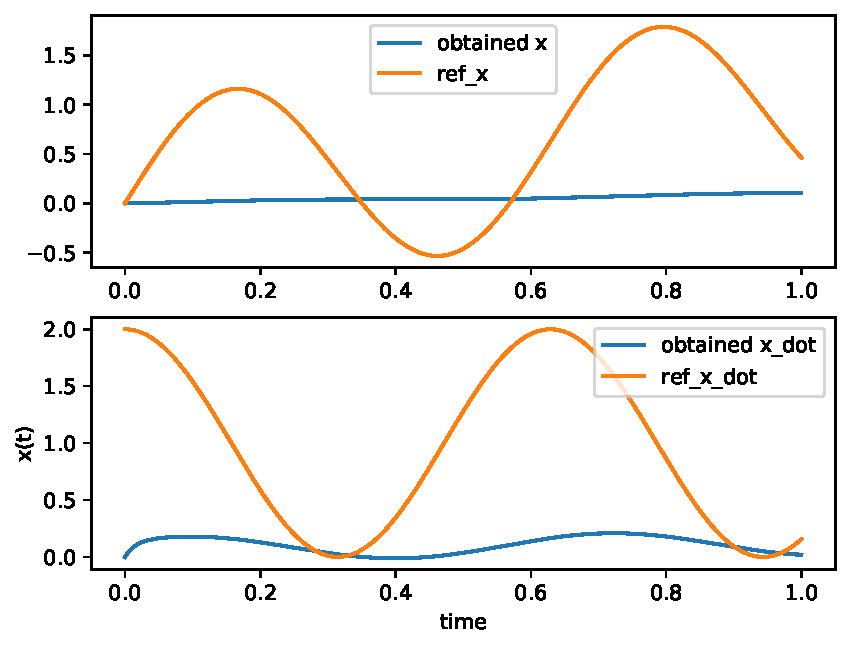
\includegraphics[width = 0.8\linewidth]{2a_tr1.pdf}
            \end{center}
            As a second reference trajectory I have chosen $x^*(t)=sin(10t)$, 
            $\dot{x}^*(t) = 10 cos(10t)$, with zero initial conditions. Here are the plots 
            of solution, obtained with $K_p = 100$, $K_d = 100$.
            \begin{center}
                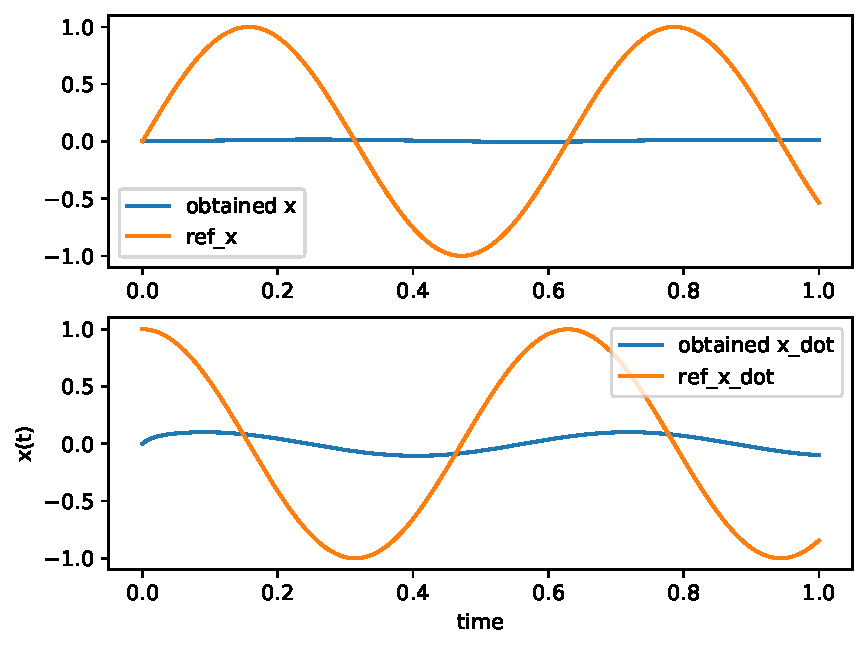
\includegraphics[width = 0.8\linewidth]{2a_tr2.pdf}
            \end{center}
            Third reference trajectory is just a step function $x^*(t)=1$, $\dot{x}^*(t) = 0$,
            with zero initial conditions. Here are the plots of solution, obtained with 
            $K_p = 5$, $K_d = 5$.
            \begin{center}
                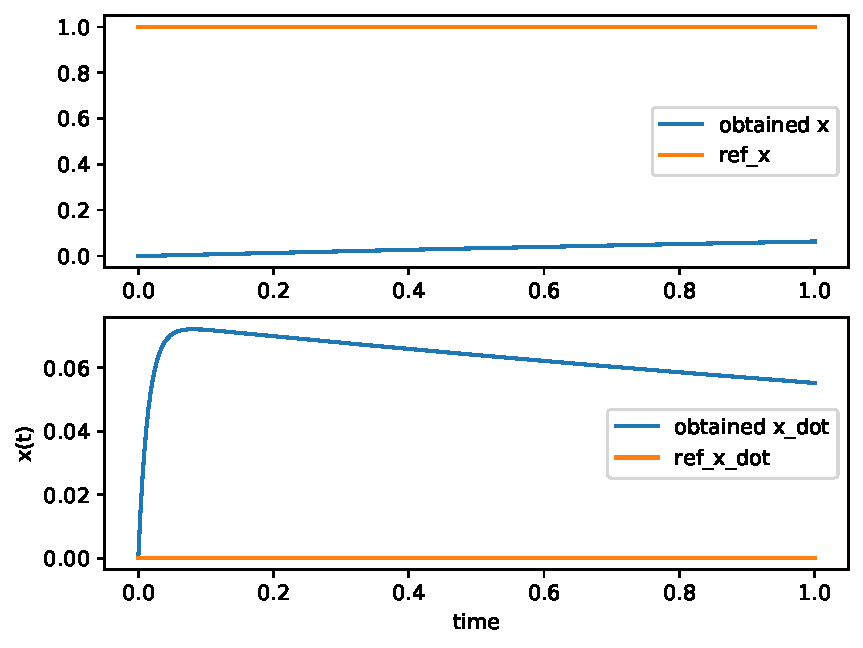
\includegraphics[width = 0.8\linewidth]{2a_tr3.pdf}
            \end{center}
            As one can see, my controller poorly follows desired trajectory and need
            to be tuned for each trajectory individually. 
    \subsection*{Part B. Controller tuning}
        We begin with $K_p = 5$, $K_d = 5$. As you can see on the above plot, 
        it gives us a large steady-state error, so $K_p$ should be increased.\\ 
        I had been increasing it, 
        until I got steady-state error $e \approx 10^{-2}$. The controller gains 
        are now $K_p = 2000$, $K_d = 5$
        \begin{center}
            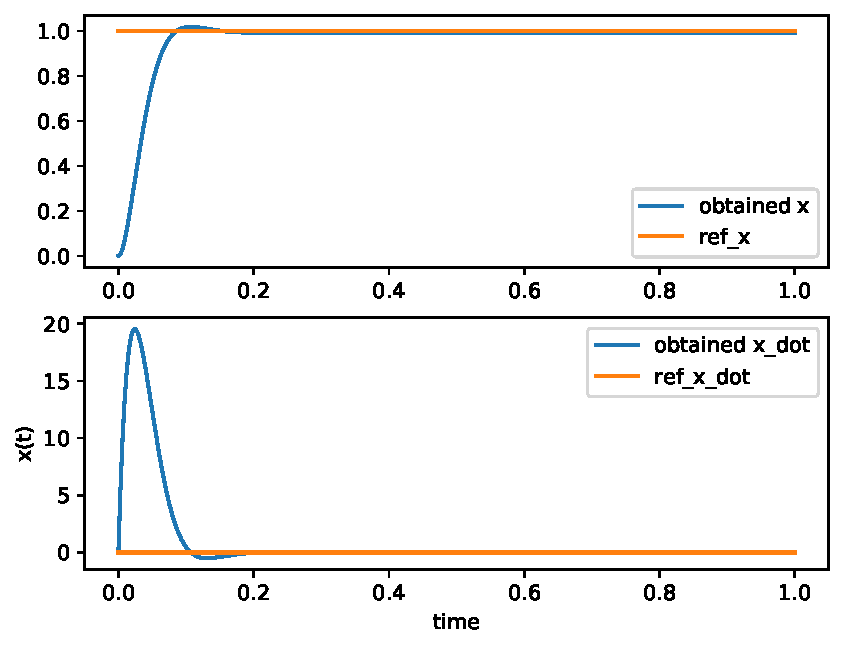
\includegraphics[width = 0.72\linewidth]{2b_1.pdf}
        \end{center}
        Now we have almost no steady-state error, but there is an overshoot appeared
        now. Therefore, $K_d$ should be increased.\\
        I had been increasing it, until I got rid of overshoot. The controller 
        gains now are $K_p = 2000$, $K_d = 13$
        \begin{center}
            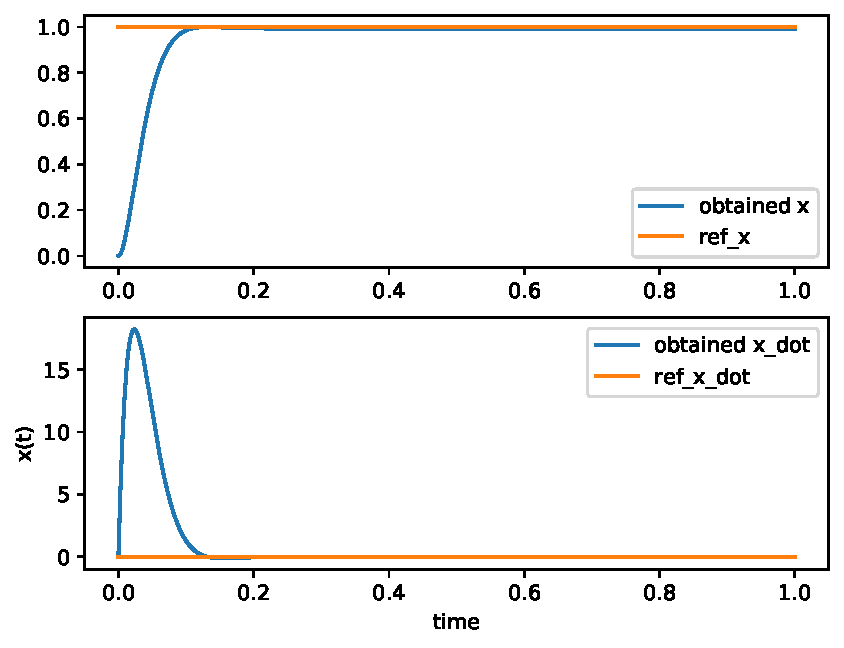
\includegraphics[width = 0.77\linewidth]{2b_2.pdf}
        \end{center}
        Now there is no overshoot, and steady-state error $e \approx 10^{-2}$, 
        as it can be seen from the plot. The gains are $K_p = 2000$, $K_d = 13$.
    \subsection*{Part C. Proving stability}
        For the controlled system 
        \begin{equation*}
            \begin{cases}
                \dot{x}=Ax+Bu\\
                u = -Kx
            \end{cases}
        \end{equation*}
        to be stable, all real parts of eigenvalues of matrix $[A-BK]$ should be
        negative. In our case, we have
        \begin{equation*}
            \begin{cases}
                \dot{x}=
                \begin{bmatrix}
                    0 & 1 \\
                    -15 & -63
                \end{bmatrix}
                x+
                \begin{bmatrix}
                    0 \\
                    1
                \end{bmatrix}
                u
                \\
                \\
                u = -
                \begin{bmatrix}
                    K_p & K_d
                \end{bmatrix}
                e
            \end{cases}
        \end{equation*}
        \begin{eqnarray*}
            A-BK = 
            \begin{bmatrix}
                0 & 1 \\
                -15 & -63
            \end{bmatrix}
            -
            \begin{bmatrix}
                0 \\
                1
            \end{bmatrix}
            \begin{bmatrix}
                2000 & 13
            \end{bmatrix}\\
            \\
            A-BK = 
            \begin{bmatrix}
                0 & 1 \\
                -15 & -63
            \end{bmatrix}
            -
            \begin{bmatrix}
                0 & 0\\
                2000 & 13
            \end{bmatrix}\\
            \\
            A-BK = 
            \begin{bmatrix}
                0 & 1 \\
                -2015 & -76
            \end{bmatrix}
        \end{eqnarray*}
        Using Matlab's \texttt{eig()} function, I obtained the eigenvalues, that 
        are
        \begin{equation*}
            eigenvalues = 
            \begin{bmatrix}
                -38 + 23.8956i\\
                -38 - 23.8956i
            \end{bmatrix}
        \end{equation*}
        As it can be seen, they have negative real parts, so the controlled system
        is stable.
    \subsection*{Part D.}
    Think of how you would implement PD control for a linear system:
    \begin{equation*}
        \begin{bmatrix}
            \dot{x_1}\\
            \dot{x_2}
        \end{bmatrix}
        = 
        \begin{bmatrix}
            10 & 3 \\
            5 & -5
        \end{bmatrix}
        \begin{bmatrix}
            x_1\\
            x_2
        \end{bmatrix}
    \end{equation*}
    This system is autonomous MIMO system. First of all, let's check its 
    stability by looking at its 
    eigenvalues, obtained with Python's \texttt{numply.linalg.eig()}.
    \begin{equation*}
        eigenvalues = 
        \begin{bmatrix}
            10.94\\
            -5.94
        \end{bmatrix}
    \end{equation*}
    As can be seen, it is unstable, because it has eigenvalue with positive
    real part. Thus, we need to add controller to the system:
    \begin{equation*}
        \dot{x} = Ax + BK_1e_1 + BK_2e_2,
    \end{equation*}
    where $K_1$ and $K_2$ are control matrices for input 1 and 2 respectively,
    $x$ is state vector, and $e_1$ and $e_2$ are two errors from two outputs. 
    Below I assumed that 
    $K_1 = K_2$ and our equation takes the form
    \begin{equation*}
        \dot{x} = Ax + BK(e_1 + e_2),
    \end{equation*}
    Applying above equation to our case:
    \begin{equation*}
        \begin{bmatrix}
            \dot{x_1}\\
            \dot{x_2}
        \end{bmatrix}
        = 
        \begin{bmatrix}
            10 & 3 \\
            5 & -5
        \end{bmatrix}
        \begin{bmatrix}
            x_1\\
            x_2
        \end{bmatrix}
        +
        \begin{bmatrix}
            1 \\
            1
        \end{bmatrix}
        \begin{bmatrix}
            K_p & K_d
        \end{bmatrix}
        \left(
            \begin{bmatrix}
                e_1\\
                \dot{e_1}
            \end{bmatrix}
            +
            \begin{bmatrix}
                e_2\\
                \dot{e_2}
            \end{bmatrix}
        \right)
    \end{equation*}
    Now let me start implementing it in Python. First, I declared some constants:
    \lstinputlisting[language = Python, firstline=6, lastline=17]{../Task2/pd1order.py}
    As we have no derivative in state vector, we should somehow calculate it. I 
    propose such formula for the derivative approximation:
    \begin{equation*}
        \dot x(t_i) = \frac{x(t_i) - x(t_{i-1})}{t_i - t_{i-1}}
    \end{equation*}
    As \texttt{odeint()} integrates numerically, it can try to compute differential
    with $\Delta t = t_i - t_{i-1}$ very small (or sometimes 0). That leads to numerical errors, and due to this
    I changed the formula to 
    \begin{equation*}
        \dot x(t_i) = \frac{x(t_i) - x(t_{i-1})}{max(t_i - t_{i-1}, 10^{-6})}
    \end{equation*}
        
    With this assumption, I can now implement differential function:
    \lstinputlisting[language = Python, firstline=22, lastline=39]{../Task2/pd1order.py}
    Integrating the solution:
    \lstinputlisting[language = Python, firstline=41, lastline=46]{../Task2/pd1order.py}
    The obtained plot of solution is presented below:
    \begin{center}
        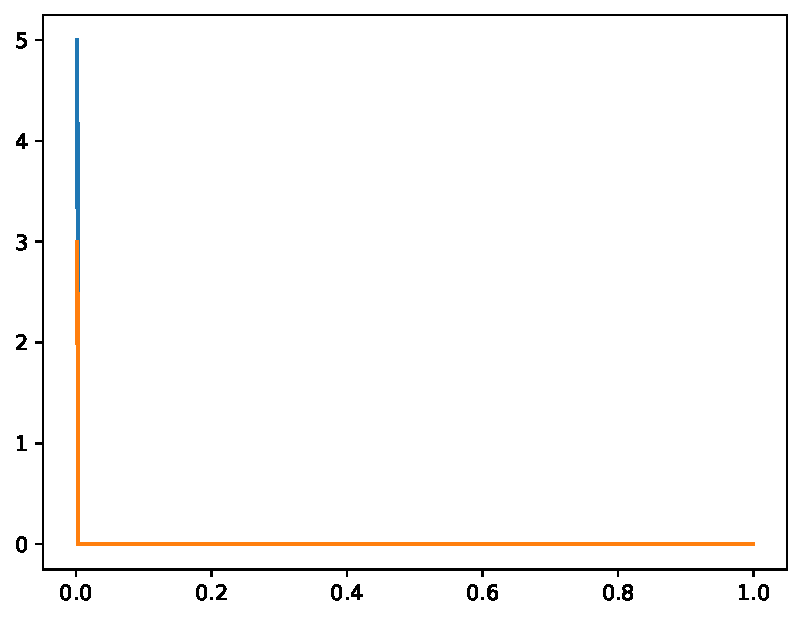
\includegraphics[width=\linewidth]{2d.pdf}
    \end{center}
    As it can be seen, the controller tries to change the system state to desired 
    one in just one time-step. That is not physically possible, and this is always
    the case, when one uses derivatives of same order as systems themselves, to control
    the systems.
    \subsection*{Part E.}
    Implement a PI/PID controller for the system: 
    $\ddot{x}+\mu \dot{x} +kx+ 9.8 = u$
    (variants are below) Test your controller on different trajectories, at 
    least two.\\
    For this task, I decided to treat the system as third order one, with $x_1 = 
    \int xdx$, $x_2 = x$, and $x_3 = \dot x$. Then, I built a state space model 
    for the system, treating the constant term $9.8$ as input.
    \begin{equation*}
        \begin{bmatrix}
            \dot{x_1}\\
            \dot{x_2}\\
            \dot{x_3}
        \end{bmatrix}
        =
        \begin{bmatrix}
            0 & 1 & 0\\
            0 & 0 & 1\\
            0 & -k & -\mu
        \end{bmatrix}
        \begin{bmatrix}
            x_1\\
            x_2\\
            x_3
        \end{bmatrix}
        + (-9.8 + u)
        \begin{bmatrix}
            0\\
            0\\
            1
        \end{bmatrix}
    \end{equation*}
    Adding our controller to control the input of the system:
    \begin{equation*}
        \begin{bmatrix}
            \dot{x_1}\\
            \dot{x_2}\\
            \dot{x_3}
        \end{bmatrix}
        =
        \begin{bmatrix}
            0 & 1 & 0\\
            0 & 0 & 1\\
            0 & -k & -\mu
        \end{bmatrix}
        \begin{bmatrix}
            x_1\\
            x_2\\
            x_3
        \end{bmatrix}
        - 9.8
        \begin{bmatrix}
            0\\
            0\\
            1
        \end{bmatrix}
        +
        \begin{bmatrix}
            0\\
            0\\
            1
        \end{bmatrix}
        \begin{bmatrix}
            K_i & K_p & K_d
        \end{bmatrix}
        \begin{bmatrix}
            e_{int}\\
            e\\
            \dot{e}
        \end{bmatrix}
    \end{equation*}
    Now let's implement the system on Python. First, I define reference functions:
    \lstinputlisting[language = Python, firstline=6, lastline=13]{../Task2/pid.py}
    These functions describe our desired trajectory. 
    In our case, $\mu = 63, k = 15$, so I defined them and some other constants:
    \lstinputlisting[language = Python, firstline=15, lastline=24]{../Task2/pid.py}
    Then I defined differential function:
    \lstinputlisting[language = Python, firstline=26, lastline=31]{../Task2/pid.py}
    As a first trajectory for testing I choose step function $x(t)=1, \dot x(t)=0$
    Here is a plot of its solution with $K_p = 100, K_i = 30, K_d = 20$
    \begin{center}
        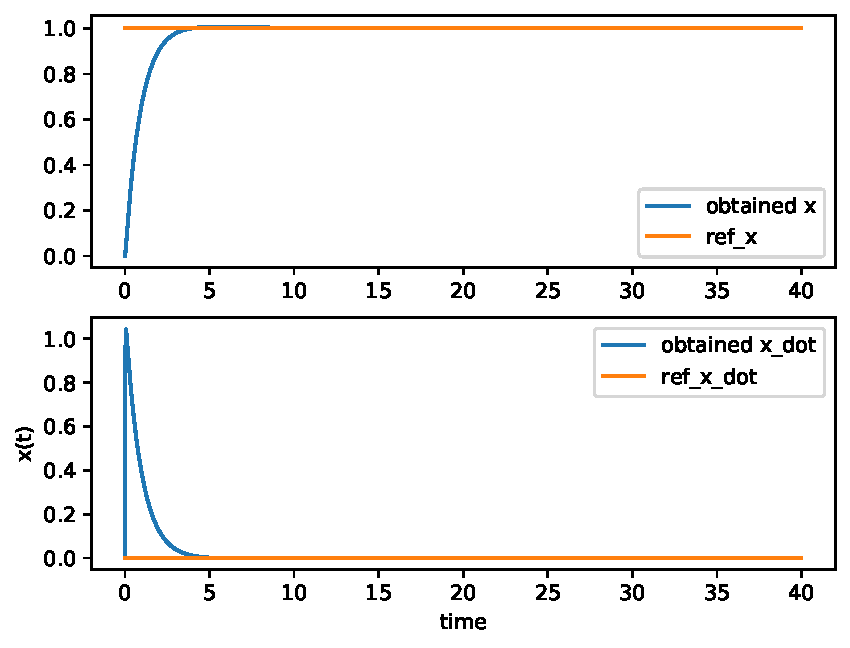
\includegraphics[width=0.8\linewidth]{PID100-30-20.pdf}
    \end{center}
    Second trajectory is $x(t)=sin(t), \dot x(t) = cos(t)$
    Here is a plot of its solution with $K_p = 100, K_i = 30, K_d = 20$
    \begin{center}
        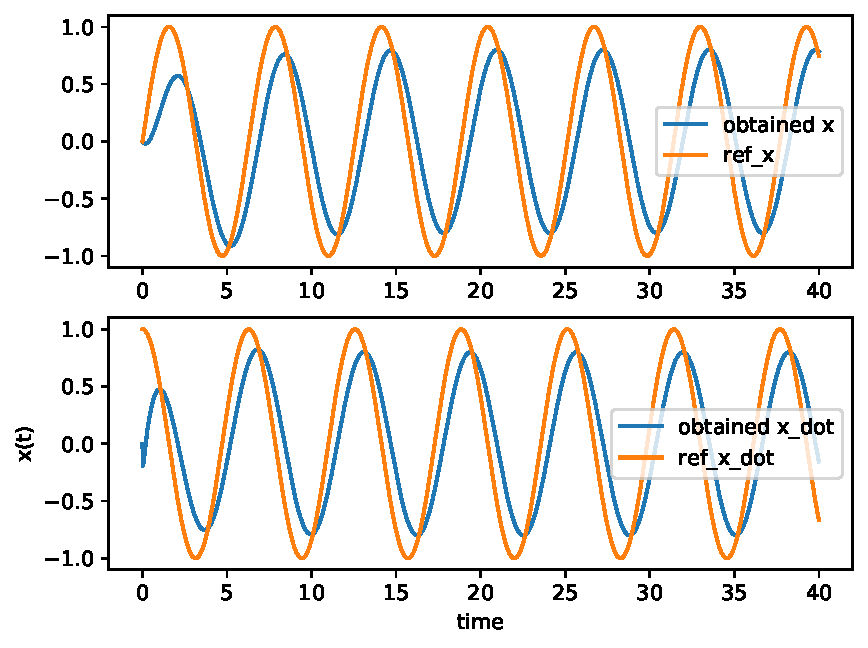
\includegraphics[width=0.8\linewidth]{2PID100-30-20.pdf}
    \end{center}
\section{Task 3. Design PID controller in Matlab}
    My system:
    \begin{equation*}
        W = \frac{s+3}{2s^3+4s^2+7s+13}
    \end{equation*}
    Step response of system without a controller:
    \begin{center}
        \includegraphics[width=0.64\linewidth]{T3Step-crop.pdf}
    \end{center}
    From the plot, it is seen, that system is marginally stable, but has oscillations
    in the beginning, and there is a steady-state error.\\
    As the first step I have built system in Simulink:
    \begin{center}
        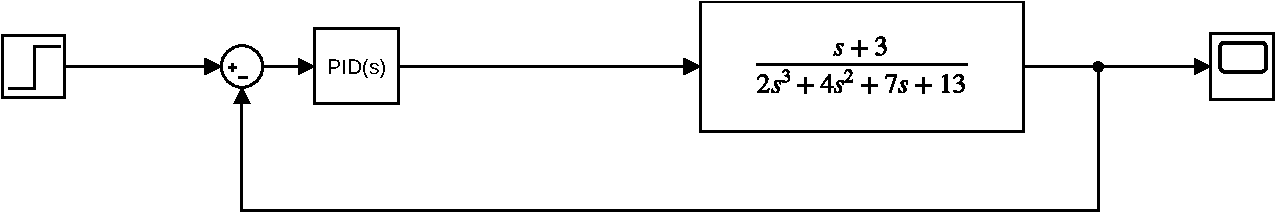
\includegraphics[width=\linewidth]{../Task3/System.pdf}
    \end{center}
    Then, I opened PID controller parameters, and used \texttt{PIDtuner} to automatically
    tune controller gains. The PID tuner have chosen $K_p = 195, K_i = 145, K_d = 20$.
    (Initial gains were fractional, but I rounded them mathematically).\\
    With these gains, step response start look like this (Note, that time scale 
    has changed!):
    \begin{center}
        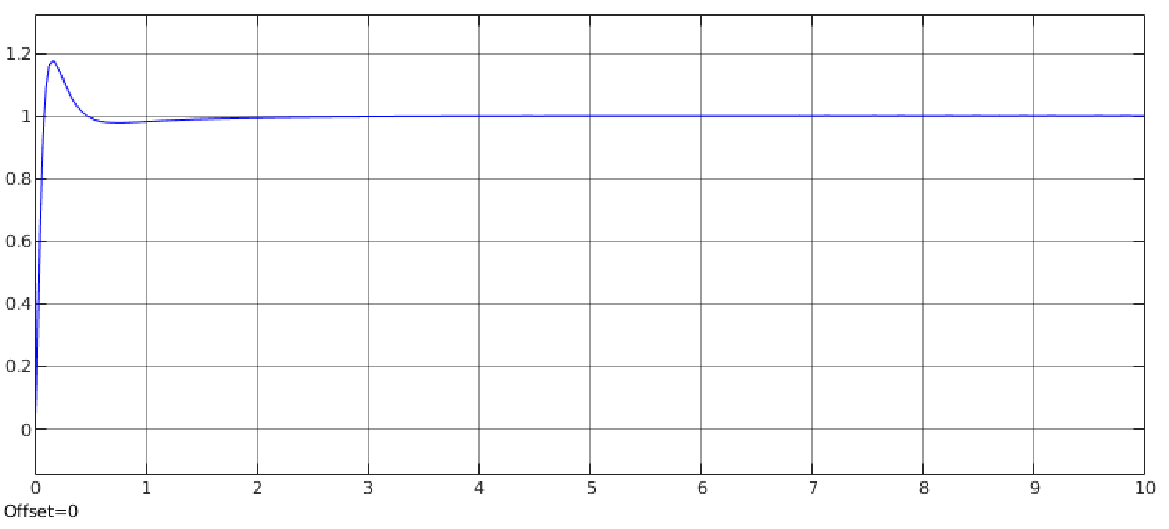
\includegraphics[width=\linewidth]{../Task3/Auto_tuned.pdf}
    \end{center} 
    After that I started to tune $K_d$ to eliminate overshoot, and obtained minimal
    overshot of $9.3\%$ with $K_d = 95$. 
    \begin{center}
        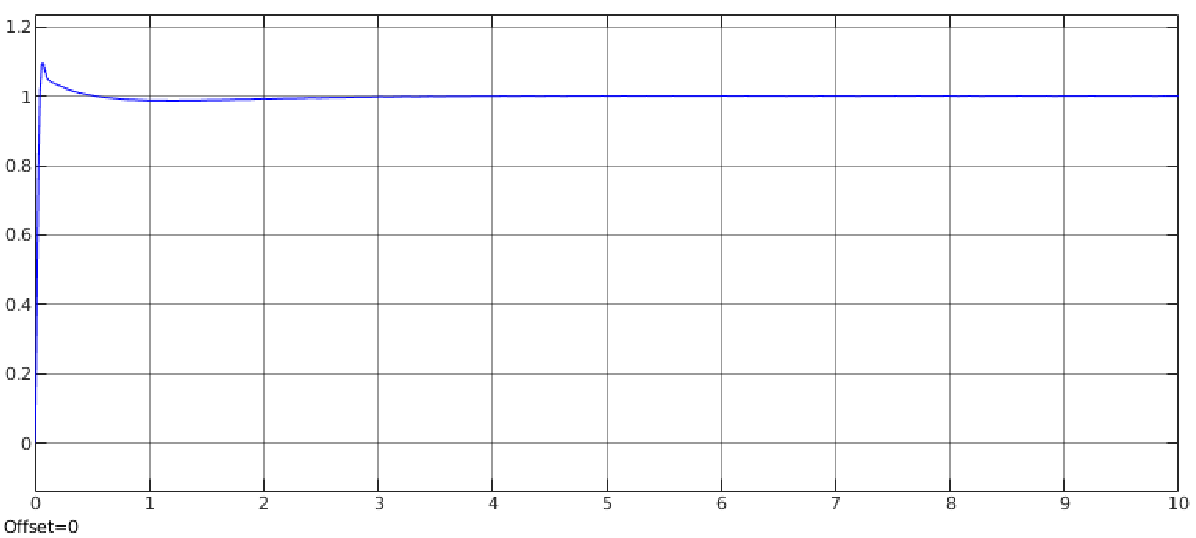
\includegraphics[width=\linewidth]{../Task3/tuned.pdf}
    \end{center}
    I decided, that such step response is quite good, and stopped there. The final 
    controller gains are $K_p = 195, K_i = 145, K_d = 20$.
\section{Task 4. Design a Lead/Lag compensator in Matlab}
    My initial system:
    \begin{equation*}
        W(s) = \frac{s^2+3s+8}{s^4+2s^3+3s^2+13s+7}
    \end{equation*}
    I entered my plant transfer function to Matlab's console with\\
    \texttt{plant = tf([1 3 8],[1 2 3 13 7])},\\
    then I opened controlSystemDesigner with \\
    \texttt{controlSystemDesigner(plant)}.\\
    From the initial plots it is visible, that my system is not stable. 
    \begin{center}
        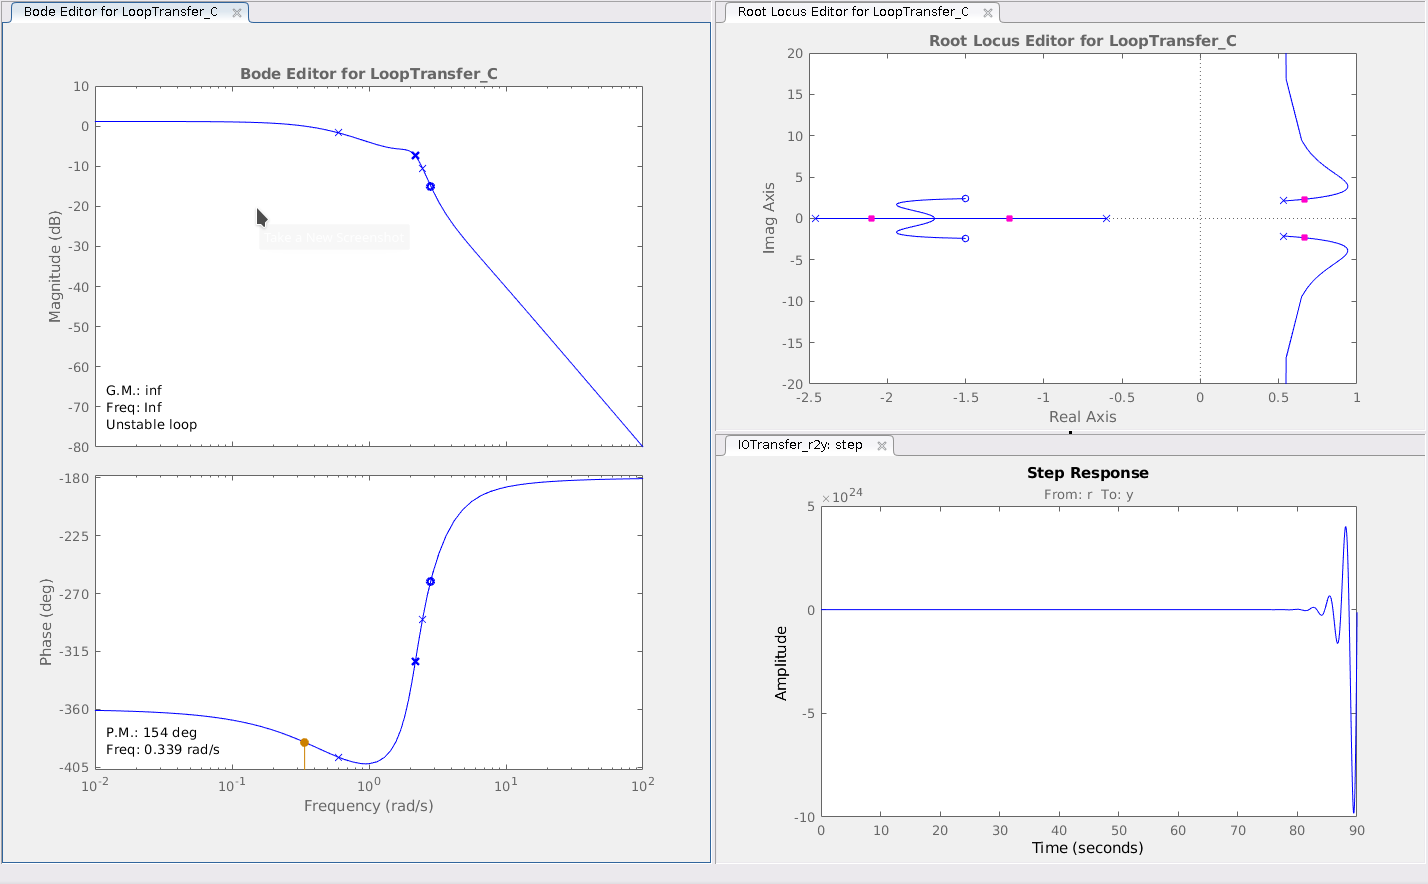
\includegraphics[width=\linewidth]{../Task4/Init.png}
    \end{center}
    First of all, we need to improve stability of the system. To do it I will add
    Lead compensator with pole at -10 and zero at -1 to shift Root-Locus right 
    in the complex plane, and increased compensator gain to 100. My lead compensator
    formula is now
    \begin{equation*}
        C(s) = 100 \frac{s+1}{s+10}
    \end{equation*}
    Here is the system step response with untuned Lead Compensator:
    \begin{center}
        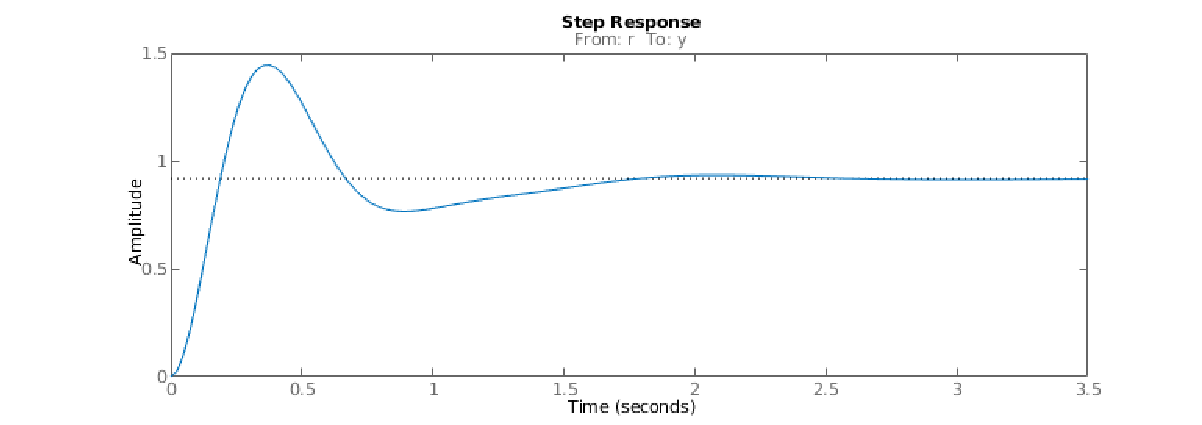
\includegraphics[width=\linewidth]{../Task4/Lead.pdf}
    \end{center}
    Then, I tuned compensator gain, pole and zero and obtained new compensator
    formula, that has better rise time, and lower overshoot.
    \begin{equation*}
        C(s) = 1125 \frac{s+0.4}{s+50}
    \end{equation*}
    The improved step response:
    \begin{center}
        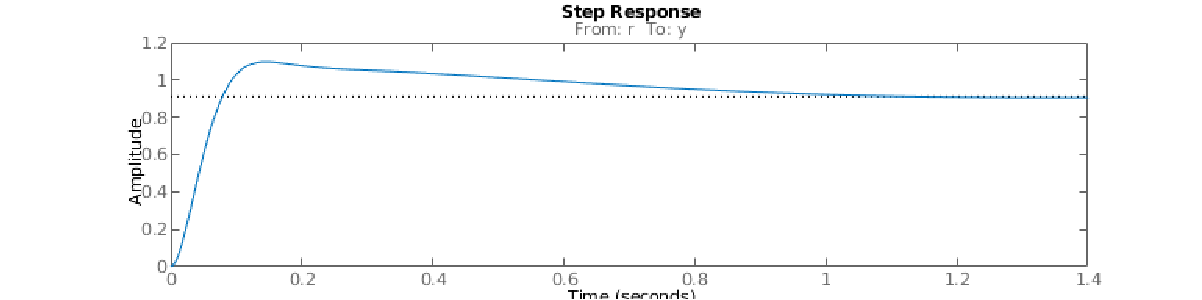
\includegraphics[width=\linewidth]{../Task4/LeadTuned.pdf}
    \end{center}
    The Lead compensator stabilized the system, give it relatively good rise time,
    low overshoot, and steady state error is almost not present. Therefore, 
    Lag Compensator for this system is not needed.
 
\section{Used software.}
\begin{itemize}
    \item Python 3.8.1
    \item Matlab R2018b 9.5.0
\end{itemize}
All software was run under Manjaro Linux with 5.4.18-rt kernel
\end{document}